


	\section{Experiment Results}
	
	%when the available clues for alignment are sparse, we have performed comparative evaluation of our model against several baselines.
	
	\subsection{Overall Performance}
	\cparagraph{Results on WBD dataset}
    Table~\ref{f1} reports the performance of all models on the WBD dataset. Since the performance of each model is very similar in two alignment directions, we will mainly discuss the results of all models in the direction of Baidu$\rightarrow$Wiki. 
    
    ITransE$'$ outperforms JE regarding all the Hits@k measures and outperforms GCN for Hits@1 in both alignment directions. This indicates that ITransE is an
outstanding model for entity alignment and it also shows that TransE can effectively embed the structure information of KGs which plays an
important role in entity alignment. However, GCN-based model performs better than ITransE in Hits@10. As aforementioned, GCNs
leverage convolutional layers to characterize an entity through careful investigations about its neighbors, including both neighboring
entities and attribute values, which can provide more fine-grained and accurate modeling and representation for the target entity.


	Comparing with GCN, the RGCN-based model further boosts the performance by 20.2\% and 24.2\% for Hits@1 and Hits@10. It shows that introducing highly multi-relational information to GCN framework can achieve significant improvements on KG embedding.
	
	Among all models, when enhanced with layer-wise highway gates, our HRGCN model performs the best, significantly improving upon RGCN by 21.0\% and 15.6\% for Hits@1 and Hits@10. This indicates that highway gates play a significant role in our model. And HGCN model which adds highway gates to GCN also improves the performance of GCN by 2.4\% and 2.3\% for Hits@1 and Hits@10. It suggests that highway gates are also beneficial to GCN. 
	
	When comparing our full model HRGCN with HRGCN (w/o $X$), we find that removing the predefined input feature matrix $X$ leads to a drop of 43.3\% for Hits@1 and 45.4\% for Hits@10. This confirms that initializing entity representations using pre-trained word embeddings and normalized value vectors is very helpful in aligning entities from different KGs.
	
	\cparagraph{Results on $\bf DBP15K_{FR-EN}$ dataset}
	Table~\ref{cross} reports Hits@1 and Hits@10 of all the compared approaches on $DBP15K_{FR-EN}$ dataset. Since we use the same French-English subset and the same split of gold standards for training and testing as in~\cite{sun2017cross}, the results of JE, MTransE, and JAPE are obtained from~\cite{sun2017cross}. JAPE has two variants: Structure Embedding (SE), Structure and attribute joint embedding (SE+AE). We also evaluate two variants of our model: HRGCN (SE) which performs semantic embedding with pre-trained word vectors, HRGCN (SE+AE) which combines semantic embedding and attribute embedding. We can see that our full model HRGCN (SE+AE) gets the best Hits@1 in both alignment directions. This indicates that our model has strong noise immunity. Although we handle cross-lingual data through rough machine translation which might introduce lots of noise, our model still outperforms all the compared baselines regarding Hits@1. JAPE (SE+AE) outperforms HRGCN (SE+AE) by 10\%$\sim$13\% for Hits@10. It shows that JAPE is an
	excellent model for entity alignmentmight. However JAPE needs additional aligned relations and attributes, while our model does not need such high-quality seed alignment data.
	
		\begin{table}
		\centering
		\small
		\begin{tabular}{c|cc|cc}
			\toprule
			\multirow{2}{*}{\bf Models} &  \multicolumn{2}{c|}{$\bf Baidu \rightarrow Wiki$} & \multicolumn{2}{c}{$\bf Wiki \rightarrow Baidu$} \\
			& \bf Hits@1 & \bf Hits@10 & \bf Hits@1 & \bf Hits@10 \\
			\midrule
			JE & 10.8 & 21.6 & 10.2 & 20.3 \\
			ITransE$'$ & 19.4 & 25.5 & 17.6 & 24.8 \\
			GCN & 17.1 & 27.3 & 15.7 & 25.9 \\
			HGCN & 19.5 & 29.6 & 19.4 & 29.5  \\
			\bf RGCN & 37.3 & 51.5 & 34.8 & 51.6 \\
			\bf HRGCN (w/o $X$) & 15.0 & 21.7 & 14.5 & 21.5 \\
			\bf HRGCN & \bf 58.3 & \bf 67.1 & \bf 57.8 & \bf 65.7 \\
			\bottomrule
		\end{tabular}
		\caption{Results comparison of entity alignment on WBD dataset.}
		\label{f1}
	\end{table}
	\begin{table}
		\centering
		\small
		\begin{tabular}{lc|cc|cc}
			\toprule
			\multicolumn{2}{c|}{\multirow{2}{*}{$\bf DBP15K_{FR-EN}$}} & \multicolumn{2}{c|}{$\bf FR \rightarrow EN$} & \multicolumn{2}{c}{$\bf EN \rightarrow FR$} \\
			& & \bf Hits@1 & \bf Hits@10 & \bf Hits@1 & \bf Hits@10 \\
			\midrule
			\multicolumn{2}{c|}{JE} & 15.38 & 38.84 & 14.61 & 37.25 \\
			\midrule
			\multicolumn{2}{c|}{MTransE} & 24.41 & 55.55 & 21.26 & 50.60 \\
			\midrule
			\multirow{2}{*}{JAPE} & SE & 29.63 & 64.55 & 26.55 & 60.30 \\
			& SE+AE & 32.39 & \bf 66.68 & 32.97 & \bf 65.91 \\
			\midrule
			\multirow{2}{*}{HRGCN} & SE & 33.43& 35.72& 31.22& 34.65\\
			& SE+AE & \bf 44.82 & 56.68 &\bf 41.08 & 52.95\\
			\bottomrule
		\end{tabular}
		\caption{Results comparison of entity alignment on $DBP15K_{FR-EN}$ dataset.}
		\label{cross}
	\end{table}
	
	%(1) The JE model outperforms the TextSim model and MLP model by 7.6\% and 4.1\%, respectively. This indicates that TransE can effectively embed the structure information of KGs which plays an important role in entity alignment. And it also suggests that the semantic information about the surface forms of entities or values can only play a supporting role, we can't rely on it completely to get the desired result.
	
	
	\subsection{Analysis}
	

\begin{table*}
	\centering
	\small
	\begin{tabular}{ccccc}
		\toprule
		\multirow{2}{*}{\bf Aligned Entities} & \bf \#Neighbors & \bf \#Similar & \bf \#Values & \bf \#Similar \\
		&\bf  Wiki \& Baidu &\bf  Neighbors &\bf  Wiki \& Baidu &\bf  Values \\
		\midrule
		Deng Jiaxian & 10 \& 33 & 5 & \ 3 \& 11 & 2\\
		Hubei Province & 21 \& 50 & 5 & 10 \& 19 & 3\\
		European Union & 66 \& 35 & 6 & 18 \& 8\ \ \ & 2\\
		%Huazhong University of & \multirow{2}{*}{11 \& 32} & \multirow{2}{*}{4} & \multirow{2}{*}{8 \& 6} & \multirow{2}{*}{1}\\
		%Science and Technology & & & & \\
		%Huazhong University of Science and Technology & 11 \& 32 & 4 & 8 \& 6 & 1 \\
		Confucius & 10 \& 20 & 4 & 7 \& 3 & 2\\
		\bottomrule
	\end{tabular}
	\caption{The statistics of example entity pairs, which our HRGCN model correctly aligns but ITransE fails.}
	\label{example}
\end{table*}
	%An extra advantage of GCN is that we can stack multiple convolution layers to capture more global and larger contextual and neighboring characteristics
	
	We further provide a detailed analysis about the experimental results.
	
	We divide the WBD test set into four subsets according to the difference between the number of neighbors of each entity pair, and compare the performance (in Hits@1) of ITransE, GCN and HRGCN on the four subsets.
	%Figure~\ref{subset} shows the $\mathrm{F}_1$ scores of on the five subsets.
	
	As shown in Figure~\ref{subset}, we can see that when the number of neighbors differs by no more than 3, all three models perform well,
	but when the difference between the entity pairs' neighborhoods becomes more prominent,
	our HRGCN model tends to deliver more clear improvement.
	%, the three models all perform well and the scores are not far-off. However, when the difference in the number of neighbors gradually increases, the gap between JE and the other two models also grows.
	\begin{figure}
	\begin{center}
		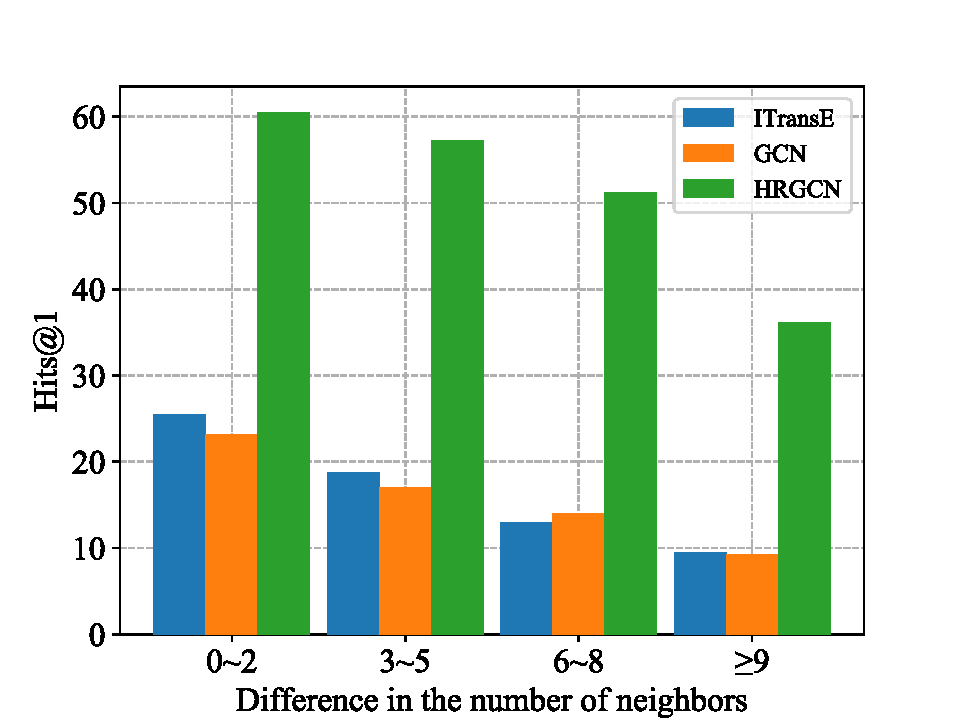
\includegraphics[width=1\linewidth]{figures/graph4.pdf}
		\caption{Hits@1 of ITransE, GCN and HRGCN on the four WBD subsets. 0$\sim$2 denotes the subset in which the number of neighbors differs from 0 to 2 for each entity pair, and similar for the remaining subsets.}
		\label{subset}
	\end{center}
\end{figure}
	\begin{figure}
		\begin{center}
			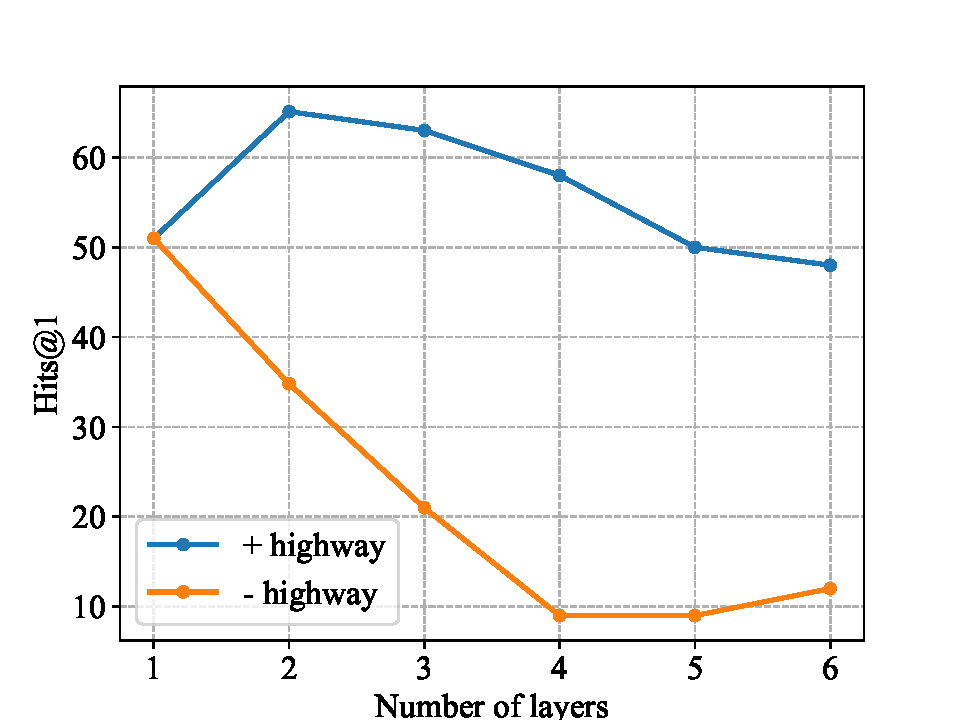
\includegraphics[width=1\linewidth]{figures/graph3.pdf}
			\caption{The effect of adding more RGCN layers in terms of Hits@1 over the test set of WBD with and without the highway gates.}
			\label{highway}
		\end{center}
	\end{figure}
	From WBD test set, we randomly choose some examples that our HRGCN model can correctly align but ITransE fails in Table~\ref{example}, as well as their neighbor information, i.e., number of neighbors, number of values, number of potentially overlapped neighbors or values for each pair.
	We can find that although several entities have dozens of neighbors in their corresponding KGs, but their similar or overlapped neighbors are quite few, showing again that
	%the number of similar neighbors of these entity pairs is no more than 6 which is very small compared to the number of their neighbors. This indicates that
	the available clues for entity alignment are sparse and ITransE may not perform well in this circumstance, while our HRGCN model can still identify useful structure information from those limited clues.
	
	%Overall, GCNs appear to be more beneficial for structure embedding than TransE, especially when the neighborhoods are very different.
	We can also observe from Table~\ref{example} that values play an important role in entity alignment.
	For instance, in the entity pair about \textit{Hubei Province}, nearly half of the neighbors for each entity are values, and among all 5 similar neighbors, 3 of them are are actually values,
	which provide crucial supporting evidence for the final prediction. Unfortunately, ITransE does not utilize those information, thus is unable to collect sufficient evidence.
	%	While the crucial information obtained from values can not be used by JE since the model dose not consider the specific values.

	
	In Figure~\ref{subset}, we can see that our HRGCN wins GCN in every subset.
	This is mainly because introducing highly multi-relational information to GCN with highway gates can help our model better embed the relational structure information and focus on the most discriminative aspects from the target entity's neighbors, thus lead to more accurate representations.
	%Figure~\ref{fig:heatmap} shows the heat maps about \textit{Centaur}'s neighbors similarities in two KGs, learned by GATs and GCNs-two, respectively.We can observe that GATs can effectively identify the potentially more similar neighbors from two KGs, which will act as discriminative evidence to support the alignment, while GCNs-two fails to distinguish those similar/discriminative neighbors from other non-relevant nodes.
		
	
	%(3) Among all models, the GAT-based model performs the best, improving upon GCNs by a margin of 1.5\%. This indicates that introducing the attention mechanism can more accurately embed the structure information. Figure~\ref{fig:heatmap} is the heat maps which show the similarities of the neighbors' embeddings (learned by GATs/GCNs) of ``Centaur'' from two KGs. We can observe that GATs effectively find the similar neighbors and there is a good distinction in the degree of similarity. However, GCNs treat them the same and the crucial similar nodes are not prominent.

	Adding more HRGCN layers can help the center entities obtain information from neighbors that are multiple hops away. However, it might also introduce noisy information from the exponentially increasing neighbors, leading to significant decline in performance as shown in Figure~\ref{highway} when no highway gates are used. We can observe that the performance of two-layered RGCNs with highway gates improves upon one-layered RGCN. Then by adding more layers the performance of highway RGCNs decreased slowly, but much slower than RGCNs without gates. This confirms that the highway gates effectively control the required balance of neighbor information transmission in RGCNs.
	
